\documentclass[10pt,UTF8]{ctexbook} %% ctexart

\title{\textbf{离散数学}讲义}
\author{钱锋\thanks{Email: strik0r\_qf@mail.nwpu.edu.cn}}

\usepackage{graphicx}
\usepackage[toc]{multitoc}
\usepackage{amsthm, amssymb, amsmath, mathrsfs, mhchem}
\usepackage{tikz,circuitikz}
\usetikzlibrary{decorations.markings, angles, quotes, arrows.meta}
\usepackage{pgfplots}
\usepackage{subcaption}
\usepackage{tikz-3dplot}
\usepackage{extpfeil}
\usepackage{diagbox}
\usepackage{float}
\usepackage{hyperref}
\hypersetup{hidelinks,
    colorlinks = true,
    allcolors = black,
    pdfstartview = Fit,
    breaklinks = true}
\usepackage{caption}
\usepackage{enumitem}
\usepackage{siunitx}
% 定义带圆圈的数字命令
\newcommand{\circled}[1]{\textcircled{\small #1}}

\usepackage{fancyhdr} % 用于自定义页眉页脚


% 设置页眉页脚样式
\fancypagestyle{plain}{%
    \fancyhf{} % 清空页眉页脚
    \fancyhead[RO,LE]{·\thepage·} % 页眉显示页码, RO表示奇数页右侧, LE表示偶数页左侧
    \fancyhead[LO]{\nouppercase{\rightmark}} % 页眉显示小节标题, LO表示奇数页左侧
    \fancyhead[RE]{\nouppercase{\leftmark}} % 页眉显示章节标题, RE表示偶数页右侧
    \renewcommand{\headrulewidth}{0.4pt} % 设置页眉横线的宽度
    \renewcommand{\footrulewidth}{0pt} % 取消页脚横线
}

\renewcommand{\headrule}{\hrule width\textwidth height\headrulewidth\vskip-\headrulewidth}

% % 取消奇偶页的页眉偏移
% \fancyhfoffset[RO,LE]{0pt}

% % 取消奇偶页的页眉偏移
% \fancyhfoffset[RO,LE]{0pt}

% 定义取消页眉的命令
\newcommand{\cancelheader}{%
    \fancyhead{} % 清空页眉
    \renewcommand{\headrulewidth}{0pt} % 取消页眉横线
    \renewcommand{\footrulewidth}{0pt} % 设置页脚横线的宽度
}

\renewcommand{\chaptermark}[1]{\markboth{第 \thechapter 章 \hspace{1em} #1}{}}
\renewcommand{\sectionmark}[1]{\markright{\thesection \, #1}}
\usepackage{titlesec} % 定义标题样式

% 设置 chapter 标题样式
\titleformat{\chapter}[hang]{\centering\heiti\Large\bfseries}{第\,\thechapter\,章}{1em}{}

% 定义 section 标题格式
\titleformat{\section}[hang]{\heiti\centering\large\bfseries}{\thesection}{1em}{}

% 定义 subsection 标题格式
\titleformat{\subsection}[hang]{\heiti\bfseries}{\textbf{\thesubsection}}{1em}{}

% 定义 subsubsection 标题格式
\setcounter{secnumdepth}{3}
\renewcommand\thesubsubsection{\arabic{subsubsection}.}
\titleformat{\subsubsection}[hang]{\kaishu}{\quad\quad\thesubsubsection\,\,}{0em}{}

% % 重新定义 textbf
% \let\oldtextbf\textbf
% \renewcommand{\textbf}[1]{{\heiti\oldtextbf{#1}}}

% % 在导言区重新定义 \normalsize 命令
% \makeatletter
% \renewcommand\normalsize{%
%    \@setfontsize\normalsize{10.5pt}{12pt}%
%    \abovedisplayskip 8\p@ \@plus2\p@ \@minus5\p@
%    \abovedisplayshortskip \z@ \@plus3\p@
%    \belowdisplayshortskip 6\p@ \@plus3\p@ \@minus3\p@
%    \belowdisplayskip \abovedisplayskip
%    \let\@listi\@listI}
% \makeatother



% 设置页边距和对齐
% \usepackage[
%     paperwidth=185mm,
%     paperheight=260mm,
%     top=35mm,
%     bottom=25mm,
%     left=18mm,
%     right=18mm,
%     footskip=15mm % 通过这里的值来调整页脚与正文内容的垂直距离
% ]{geometry}

\usepackage[
    paperwidth=210mm,
    paperheight=297mm,
    top=40mm,
    bottom=31.8mm,
    left=25.4mm,
    right=25.4mm,
    footskip=15mm % 通过这里的值来调整页脚与正文内容的垂直距离
]{geometry}

% \usepackage[
%     paperwidth=195mm,
%     paperheight=270mm,
%     top=40mm,
%     bottom=25mm,
%     left=23.5mm,
%     right=23.5mm,
%     footskip=15mm % 通过这里的值来调整页脚与正文内容的垂直距离
% ]{geometry}
\usepackage{mdframed}
\mdfsetup{
  linewidth=0.4pt,
  frametitlebackgroundcolor=white, % 或者 transparent
  frametitlefont=\heiti\bfseries,
  frametitleaboveskip=10pt,
  frametitlebelowskip=5pt,
  frametitlealignment=\raggedright % 新增此行
}
\usepackage{fontspec}
% 设置 Menlo 字体
\setmonofont{Menlo}
\usepackage{fancyvrb}
\usepackage{xcolor}
\usepackage{listings}

% \definecolor{string}{HTML}{067D17}
% \definecolor{comment}{HTML}{8C8C8C}
% \definecolor{keyword}{HTML}{0033B3}
% \definecolor{class_field}{HTML}{871094}

\lstset{breaklines}
%这条命令可以让LaTeX自动将长的代码行换行排版
\lstset{extendedchars=false}
%这一条命令可以解决代码跨页时,章节标题,页眉等汉字不显示的问题
\lstset{escapeinside={(*}{*)}}

\lstset{
    basicstyle=\small\ttfamily\heiti,
    numbers=left,
    numberstyle=\scriptsize\fontspec{Menlo}, % 使用 Menlo 字体
    stepnumber=1,
    numbersep=8pt,
    frame=leftline,
    xleftmargin=2em, % 调整代码块的左边界
    framexleftmargin=0pt, % 调整边框的位置
    breaklines=true,
    % postbreak=\mbox{\textcolor{red}{$\hookrightarrow$}\space},
    % keywordstyle=\bfseries\color{keyword},          % keyword style
    % commentstyle=\heiti\color{comment},       % comment style
    % stringstyle=\color[HTML]{067D17},
    showstringspaces=false,
    % string literal style
    % escapeinside={\%*}{*)},            % if you want to add LaTeX within your code
    % morekeywords={}               % if you want to add more keywords to the set
}

\usepackage{smartdiagram}
\usepackage{subcaption}
\everymath{\displaystyle}

\begin{document}

\newtheoremstyle{mytheoremstyle}
    {1.5ex}                                         % Space above
    {1.5ex}                                         % Space below
    {}                                              % Font for body
    {}                                              % Indent amount
    {\bfseries}                                     % Font for head
    {}                                              % Punctuation after head
    {0.5em plus 0.2em minus 0.1em}                  % Space after head
    {\thmname{#1}\thmnumber{ #2}.\thmnote{ (#3).}}

\theoremstyle{mytheoremstyle} \newtheorem{definition}{定义}[section]
\theoremstyle{mytheoremstyle} \newtheorem{example}{习题}[section]
\theoremstyle{mytheoremstyle} \newtheorem{exercise}{}[]

\newtheoremstyle{my2theoremstyle}
    {1.5ex}                                         % Space above
    {1.5ex}                                         % Space below
    {\kaishu}                                              % Font for body
    {}                                              % Indent amount
    {\bfseries}                                     % Font for head
    {}                                              % Punctuation after head
    {0.5em plus 0.2em minus 0.1em}                  % Space after head
    {\thmname{#1}\thmnumber{ #2}.\thmnote{ (#3).}}

\theoremstyle{my2theoremstyle}
\newtheorem{thm}{定理}[section]
\newtheorem{law}{定律}[section]
\newtheorem{educt}{推论}
\newtheorem{prop}{命题}
\newtheorem{lemma}{引理}
\newtheorem{axiom}{公理}
\newtheorem{property}{性质}

\newtheoremstyle{my4theoremstyle}
    {1.5ex}                                         % Space above
    {1.5ex}                                         % Space below
    {}                                              % Font for body
    {}                                              % Indent amount
    {\bfseries}                                     % Font for head
    {}                                              % Punctuation after head
    {0.5em plus 0.2em minus 0.1em}                  % Space after head
    {\thmname{#1}.}

\theoremstyle{my4theoremstyle} \newtheorem*{sol}{解}

\newtheoremstyle{my3theoremstyle}
    {1.5ex}                                         % Space above
    {1.5ex}                                         % Space below
    {}                                              % Font for body
    {}                                              % Indent amount
    {\kaishu}                                       % Font for head
    {}                                              % Punctuation after head
    {0.5em plus 0.2em minus 0.1em}                  % Space after head
    {\thmname{#1}\thmnumber{ #2}.\thmnote{ (#3).}}

\theoremstyle{my3theoremstyle} \newtheorem*{remark}{注}

\begin{titlepage}
    \thispagestyle{empty}
    \centering
        \vspace*{2cm}
        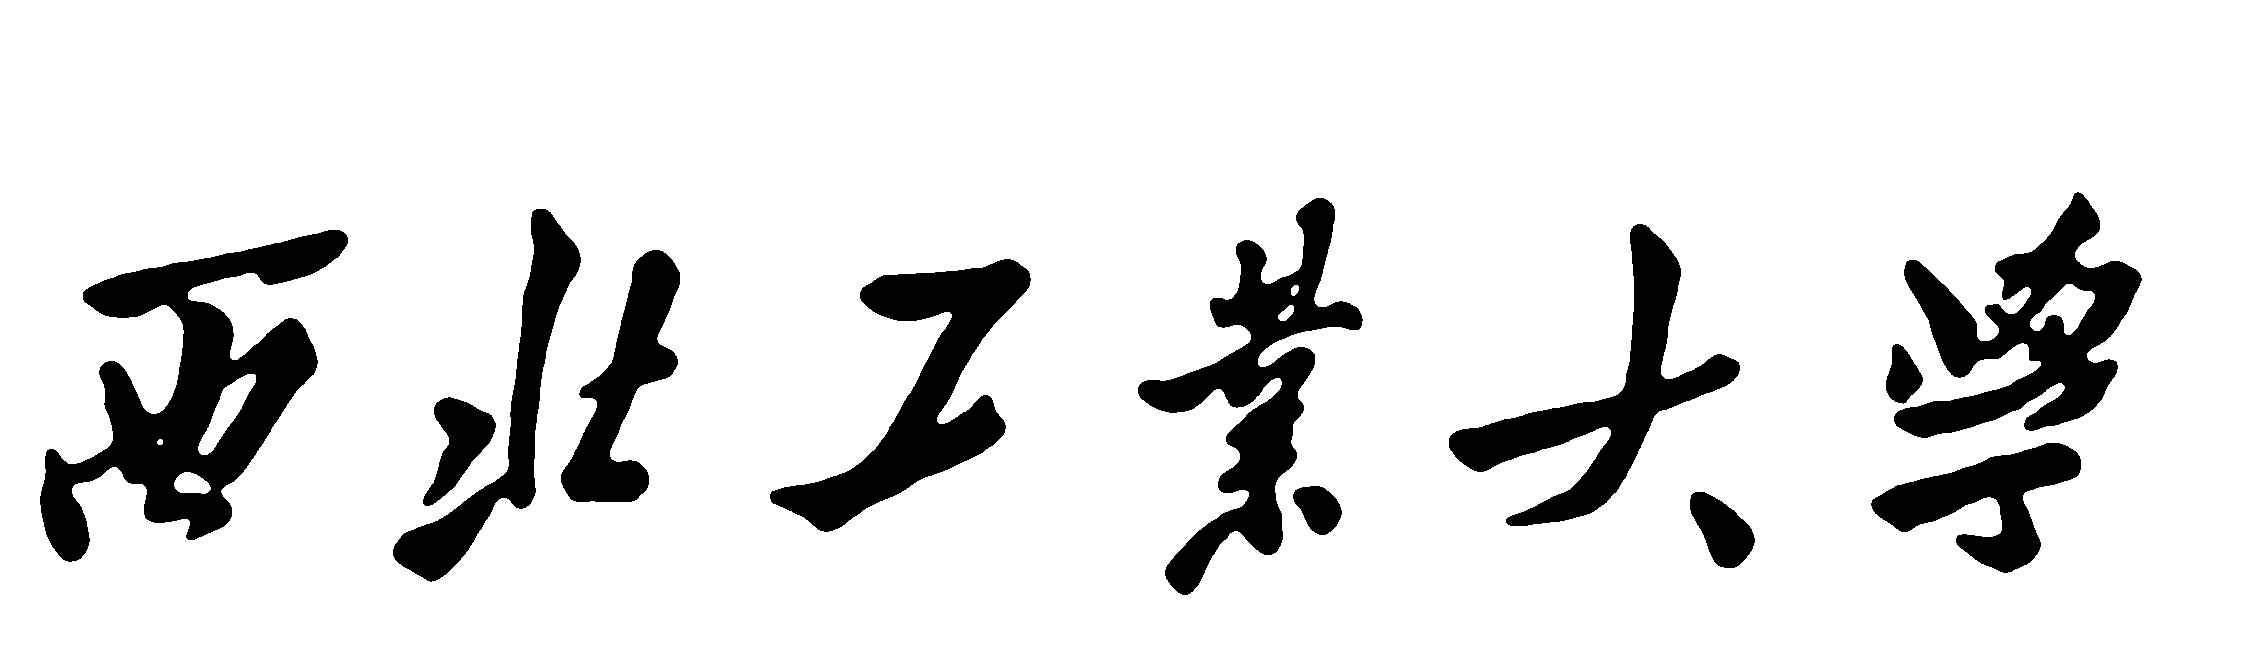
\includegraphics[width=0.5\textwidth]{pic/npu_2.png}\par
        \vspace{1cm}
        
\includegraphics[width=0.5\textwidth]{pic/npu_1.png}\par
    \vspace{1cm}
        \begin{center}
            \Huge \heiti \textbf{计算机网络作业集}

            Computer Networking
        \end{center}
        \vspace{5cm}
        \begin{center}
        \songti
        \kaishu 软件学院 \, \heiti\textbf{钱锋} \quad \songti 编
        \vspace{0.5cm}

    \today
    \end{center}
\end{titlepage}

\frontmatter
\newpage
\pagestyle{plain}
\makeatother

% \input{丛书前言.tex}
\chapter{前言}
\thispagestyle{empty}

\quad\quad 这本作业集的结构是按照教材 \cite{自顶向下} 的章节结构来划分的,
请老师在批改的时候通过目录定位到对应的章节作业. 此外, 由于作业设计的习题只是
教材习题中的一部分, 因此题号与教材上略有差异——本作业集的习题按照其在教材上的
顺序, 从 1 开始重新编号.

\begin{flushright}
    \kaishu
    钱锋

    \includegraphics*[width = 20mm]{pic/npu_2.png}
    \raisebox{0.5\height}{软件学院}

    2024 年 3 月
    \songti
\end{flushright}

\newpage
\thispagestyle{empty}

% 设置目录页的页码格式
\addtocontents{toc}{\protect\thispagestyle{empty}}
\pagestyle{plain}
{\tableofcontents}
\newpage
\thispagestyle{empty}
\cleardoublepage % 确保正文从奇数页开始


% 设置章节标题页的页眉和页脚为空白页样式
\makeatletter
\let\ps@plain\ps@empty
\makeatother

\mainmatter

\chapter{计算机网络和因特网}

\section{习题}

% \begin{example}
%     考虑一个应用程序以稳定的速率传输数据 (例如, 发送方每 $k$ 个时间单元产生一个 
%     $N$ 比特的数据单元, 其中 $k$ 较小且固定). 另外, 当这个应用程序启动时, 
%     它将连续运行相当长的一段时间. 据此回答下列问题:
%     \begin{enumerate}[label={$\left.\mathrm{\alph*}\right)$}, itemsep=0pt]
%         \item 是分组交换还是电路交换网更适合这种应用? 为什么?
%         \item 假定使用了分组交换网, 并且该网中的所有流量都来自如上所述的这种
%         应用程序.
%         此外, 假定该应用程序数据传输速率的综合小于每条链路的各自容量. 
%         需要某种形式的拥塞控制吗? 为什么?
%     \end{enumerate}
% \end{example}

\begin{example}
    考虑两台主机 A 和 B 有一条速率为 $R$ (bps) 的链路相连. 假定这两台主机相隔 $m$ (m),
    沿该链路的传播速率为 $s$ (m/s). 主机 A 向主机 B 发送长度为 $L$ (bit) 的分组.
    \begin{figure}[H]
        \centering




        \tikzset{every picture/.style={line width=0.75pt}} %set default line width to 0.75pt        

        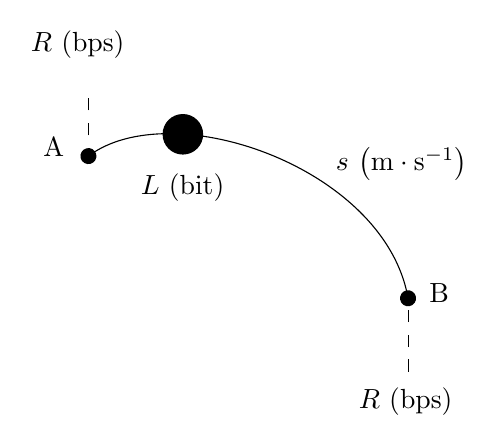
\begin{tikzpicture}[x=0.75pt,y=0.75pt,yscale=-1,xscale=1]
        %uncomment if require: \path (0,300); %set diagram left start at 0, and has height of 300
        
        %Curve Lines [id:da6142230575174562] 
        \draw    (100,118) .. controls (140,88) and (243,123.5) .. (254,186.5) ;
        \draw [shift={(254,186.5)}, rotate = 80.1] [color={rgb, 255:red, 0; green, 0; blue, 0 }  ][fill={rgb, 255:red, 0; green, 0; blue, 0 }  ][line width=0.75]      (0, 0) circle [x radius= 3.35, y radius= 3.35]   ;
        \draw [shift={(100,118)}, rotate = 323.13] [color={rgb, 255:red, 0; green, 0; blue, 0 }  ][fill={rgb, 255:red, 0; green, 0; blue, 0 }  ][line width=0.75]      (0, 0) circle [x radius= 3.35, y radius= 3.35]   ;
        %Shape: Circle [id:dp6246733531959744] 
        \draw  [fill={rgb, 255:red, 0; green, 0; blue, 0 }  ,fill opacity=1 ] (136,107.5) .. controls (136,102.25) and (140.25,98) .. (145.5,98) .. controls (150.75,98) and (155,102.25) .. (155,107.5) .. controls (155,112.75) and (150.75,117) .. (145.5,117) .. controls (140.25,117) and (136,112.75) .. (136,107.5) -- cycle ;
        %Straight Lines [id:da5479562393534617] 
        \draw  [dash pattern={on 4.5pt off 4.5pt}]  (100,120) -- (100,84.5) ;
        
        %Straight Lines [id:da2224114279600633] 
        \draw  [dash pattern={on 4.5pt off 4.5pt}]  (254,222) -- (254,186.5) ;
        
        % Text Node
        \draw (77,108) node [anchor=north west][inner sep=0.75pt]   [align=left] {A};
        % Text Node
        \draw (263,178) node [anchor=north west][inner sep=0.75pt]   [align=left] {B};
        % Text Node
        \draw (124,125.4) node [anchor=north west][inner sep=0.75pt]    {$L\mathrm{\ ( bit)}$};
        % Text Node
        \draw (71,56.4) node [anchor=north west][inner sep=0.75pt]    {$R\mathrm{\ ( bps)}$};
        % Text Node
        \draw (229,228.4) node [anchor=north west][inner sep=0.75pt]    {$R\mathrm{\ ( bps)}$};
        % Text Node
        \draw (218,112.4) node [anchor=north west][inner sep=0.75pt]    {$s\mathrm{\ \left( m\cdot s^{-1}\right)}$};
        
        
        \end{tikzpicture}
    \end{figure}
    \begin{enumerate}[label={$\left.\mathrm{\alph*}\right)$}, itemsep=0pt]
        \item 用 $m$ 和 $s$ 来表示传播时延 $d_\mathrm{prop}$.
        \begin{sol}
            根据传播时延的定义可知, 传播时延是节点间距离与传播速度的比值, 即
            $d_\mathrm{prop} = m/s$.
        \end{sol}
        \item 用 $L$ 和 $R$ 来表示该分组的传输时间 $t_\mathrm{trans}$.
        \begin{sol}
            传输时延是指数据从节点被推入通信链路中所花的时间,
            它是数据长度与链路传输速率的比值, 因此 $d_\mathrm{trans} = L/R$.
            % 由于数据传输到 B 节点后进入主机 B 也需要时间, 因此本题中所要求的时间\footnote{
            %     为了避免混淆, 原题目中的传播时间 $d_\mathrm{trans}$ 
            %     在此处记作 $t_\mathrm{trans}$, 记号 $d_\mathrm{trans}$ 
            %     仅用来表示一个分组穿过节点与链路的分界面的时间, 下同.
            % }
            % $t_\mathrm{trans} = 2d_\mathrm{trans} = 2L/R$.
        \end{sol}
        \item 忽略处理和排队时延, 得出端到端时延的表达式.
        \begin{sol}
            在该问题中, 端到端时延由传输时延和传播时延两部分组成, 而这两个部分
            在前两问中都已经计算过了, 因此
            \[ d_\mathrm{end-end} = d_\mathrm{prop} + d_\mathrm{trans}
            = \dfrac{m}{s} + \dfrac{L}{R}. \]
        \end{sol}
        \item 假定主机 A 在时刻 $t=0$ 开始传输该分组, 在时刻 $t = t_\mathrm{trans}$,
        该分组的最后一个比特在什么地方?
        \begin{sol}
            该时刻已经经历了一个传输时延, 即第一个分组已经完全传输到链路当中了.
            该分组的最后一个比特在链路中已经传播了 $d_\mathrm{trans} - d_\mathrm{trans}
            = 0$ 的时间. 在这段时间内其走过的距离为
            \[ l = s \times 0 = 0, \]
            即此时该分组的最后一个比特位于链路的 A 端点处.
        \end{sol}
        \item 假定 $d_\mathrm{prop}$ 大于 $d_\mathrm{trans}$. 
        在时刻 $t = d_\mathrm{trans}$, 该分组的第一个比特在何处?
        \begin{sol}
            根据已知条件, 该时刻该分组的第一个比特依然在链路中传播,
            由于第一个比特是直接进入链路开始传播的, 因此它已经传播了
            $d_\mathrm{trans}$ 个单位时间, 于是它所处的位置是
            $l = sd_\mathrm{trans} = sL/R$.
        \end{sol}
        \item 假定 $d_\mathrm{prop}$ 小于 $d_\mathrm{trans}$. 
        在时刻 $t = d_\mathrm{trans}$, 该分组的第一个比特在何处?
        \begin{sol}
            根据已知条件, 该时刻第一个比特已经到达 B 主机了.
        \end{sol}
    \end{enumerate}
\end{example}

\begin{example}
    考虑从主机 A 向主机 B 通过分组交换网发送语音 (VoIP). 主机 A 将模拟语音
    转换为传输中的 64kbps 数字比特流, 然后主机 A 将这些比特分为 56 字节的分组.
    A 和 B 之间有一条链路: 它的传输速率是 2Mbps, 传播时延是 10ms. 一旦 A 收集
    了一个分组, 就将它向主机 B 发送. 一旦主机 B 接收到一个完整的分组, 它将该
    分组的比特转换成模拟信号. 从比特产生 (从位于主机 A 的初始模拟信号起) 的时刻起,
    到该比特被解码 (在主机 B 上作为模拟信号的一部分), 花了多少时间?
    \begin{sol}
        我们先统一单位, 统一用比特作为单位来进行计算. 于是, 主机 A 发送的每个分组
        的大小为 $56 \times 8 = 448\si{b}$.
        这就是说, 主机 A 只需要 $448/64000$ 秒就能产生一个完整的分组, 这就是
        传输过程中的处理时延. 这就是说,
        \[ d_\mathrm{proc} 
        = \dfrac{56\si{B}}{64 \si{kbps}}
        = \dfrac{56 \times 8 \si{b}}{64 \times 10^3 \si{b \cdot s^{-1}}}
        = 7 \times 10^{-4} \si{s} =0.7 \si{ms}. \]
        \newline 接下来考虑传输时延, 事实上, 根据传输时延的定义,
        \[ d_\mathrm{trans} 
        = \dfrac{56\si{B}}{2\si{Mbps}}
        = \dfrac{56 \times 8 \si{b}}{2 \times 10^6 \si{b \cdot s^{-1}}}
        = 2.24 \times 10^{-4} \si{s} = 0.224 \si{ms}. \]
        \newline 于是最终的端到端时延为
        \[ d_\mathrm{end-end} = d_\mathrm{proc} + d_\mathrm{trans} +
        d_\mathrm{prop} = 0.7\si{ms} + 0.224 \si{ms} + 10\si{ms}
        = 10.924 \si{ms}. \]
    \end{sol}
\end{example}

\begin{example}
    假设用户共享一条 3Mbps 的链路. 又设每个用户传输时要求 150kbps, 但是
    每个用户仅有 10\% 的时间传输.
    \begin{enumerate}[label={$\left.\mathrm{\alph*}\right)$}, itemsep=0pt]
        \item 当使用电路交换时, 能够支持多少用户?
        \begin{sol}
            使用电路交换时, 每个用户都会占用一定的带宽, 因此我们可以直接用
            链路带宽和用户需求做商, 则
            \[ \mathrm{userNum} = \dfrac{3 \si{Mbps}}{150 \si{kbps}}
            = \dfrac{3 \times 10^6 \si{bps}}{150 \times 10^3 \si{bps}}
            = 20, \]
            因此在使用电路交换时, 能够支持最多 20 名用户.
        \end{sol}
        \item 当使用分组交换时, 用户正在传输的概率为?
        \begin{sol}
            由于每个用户只有 10\% 的时间传输, 所以其正在传输的概率为 0.1.
        \end{sol}
        \item 假设使用分组交换, 且有 120 名用户. 在任何给定时刻, 实际有 $n$
        个用户正在传输的概率是?
        \begin{sol}
            显然, 我们可以将这个问题视为连续进行 120 次随机事件发生概率为 0.1 
            的 Bernoulli 试验,
            正在传输数据的用户数量 $X \sim B(0.1, 120)$. 那么
            \[ P(X = n) = \mathrm{C}_{120}^n \times 0.1^n
            \times 0.9{120-n}. \]
            其中 $\mathrm{C}_m^k = \binom{m}{k}$ 为组合数, 即有限集合 $A$
            ($A$ 中含有 $m$ 个元素, 记作 $|A| = m$)
            的满足 $|S| = k$ 的子集 $S \subset A$ 的数量.
        \end{sol}
    \end{enumerate}
\end{example}

\begin{example}
    在一个电路交换网络中, 每台端系统与一台交换机直接相连, 当两台端系统要通信时, 该网络在两台
    端系统之间建立一条专用的端到端连接.
    用户在忙时以 1000kbps 的速率产生数据, 但忙时仅以 $p=0.1$ 的概率产生数据,
    假定电路交换链路的带宽为 1Gbps.
    \begin{enumerate}[label={$\left.\mathrm{\alph*}\right)$}, itemsep=0pt]
        \item 在采用电路交换技术时, 能被支持的最大用户数量 $N$ 是多少?
        \begin{sol}
            可以用链路带宽与用户需求带宽做商直接得到能够支持的最大用户数量
            \[ N = \dfrac{1\si{Gbps}}{100\si{kbps}}
            = \dfrac{1 \times 10^9 \si{bps}}{100 \times 10^3 \si{bps}}
            = 10^4. \]
        \end{sol}
        \item 在使用分组交换时, 假设有 $M$ 个用户, 多于 $N$ 个用户发送数据
        的概率为?
        \begin{sol}
            设正在发生数据的用户数量为 $X$, 显然 $X \sim B(0.1, M)$. 同时,
            由于两个用户发送数据与否是独立的, 因此
            随机事件 $\left\{ X=N+1 \right\},
            \left\{ X=N+2 \right\},
            \cdots,
            \left\{ X=M \right\}$
            是随机事件 $\left\{ X>N \right\}$ 的一个划分, 由全概率公式得
            \[ P(X>N) = \sum_{k=N+1}^{M} P(X=k)
            = \sum_{k=N+1}^{M} \mathrm{C}_M^k \times 0.1^k \times 0.9^{M-k}. \]
        \end{sol}
    \end{enumerate}
\end{example}

\begin{example}
    令 $a$ 表示在一条链路上分组的到达率, 其单位为 $\si{pkt/s}$, $\mu$ 为
    一条链路上分组的传输率, 基于 $d = d_\mathrm{queue} + d_\mathrm{trans}$,
    用 $a$ 和 $\mu$ 表示 $d$.
    \begin{sol}
        要用 $a$ 和 $\mu$ 表示 $d$, 只需用 $a$ 和 $\mu$ 表示
        $d_\mathrm{queue}$ 和 $d_\mathrm{trans}$. 我们只考虑 $1$ 个分组, 那么
        \[ d_\mathrm{queue} = \dfrac{1}{a}, \quad 
        d_\mathrm{trans} = \dfrac{1}{\mu}. \]
        于是总时延
        \[ d = \dfrac{1}{a} + \dfrac{1}{\mu}. \]
    \end{sol}
\end{example}

Little 公式是排队论中的一个著名公式, 设 $N$ 是传输队列中待传输分组的平均数量,
$a$ 为分组到达率, $d$ 为一个分组经历的平均总时延 (即排队时延加传输时延).
Little 公式表明,
\[ N = ad. \]
其实呢, Little 公式的意思就是说, 每分钟有 $a$ 个人来排队,
处理一个人平均需要 $d$ 分钟, 那么这个队伍的长度就应该是 $ad$.




\begin{example}
    考虑一台路由器缓存前面的一条出链路. 假定某队列平均包含 10 个分组, 
    平均分组排队时延是 10ms, 链路传输速率为 100pkt/s.
    不考虑丢包情况, 使用 Little 公式计算平均分组到达率.
    \begin{sol}
        由已知条件, $N = 10$, $d_\mathrm{queue} = 10\si{ms}$,
        $d_\mathrm{trans} = \dfrac{1}{100} \si{s}$, 那么
        \[ N = a d 
        = a \left( d_\mathrm{queue} + d_\mathrm{trans} \right), \]
        代入数值,
        \[ 
        \begin{aligned}
            10 \si{pkt} 
            &= a \si{pkt/s} \left(
                10\si{ms} + \dfrac{1}{100}\si{s}
            \right) 
            = a \si{pkt/s} \left(
                \dfrac{1}{100} \si{s} + \dfrac{1}{100}\si{s}
            \right) \\ 
            & = a \times 0.02 \si{s},
        \end{aligned} \]
        解得平均分组到达率 $a = 10/0.02 = 500 \si{pkt/s}$.
    \end{sol}
\end{example}

\begin{example}
    假设你希望从波士顿向洛杉矶紧急传送 $40 \times 10^{12} \si{B}$ 的数据,
    你有一条 $1\si{Gbps}$ 的专用链路可用于传输数据. 你是愿意通过这条链路传输
    数据, 还是愿意使用 FedEx 夜间快递来交付?
    \begin{sol}
        FedEx 夜间快递是指 FedEx 提供的在晚间送达包裹的服务,
        这种服务通常适用于那些需要在次日早晨或者特定时间内送达的包裹\footnote{
            这段材料由 ChatGPT 生成, ChatGPT 可能会生成错误的信息, 请谨慎参考.
        }. 
        我们不妨假设 FedEx 可以在 72 小时内将包裹送达洛杉矶.
        那么使用专用链路的传输时间 
        \[ 
        \begin{aligned}
            t &= \dfrac{40 \times 10^{12} \si{B}}{1 \si{Gbps}}
            = \dfrac{8 \times 40 \times 10^{12} \si{b}}{10^9 \si{bps}} \\ 
            &= 320,000 \si{s} = \dfrac{320,000 \si{s}}{3600 \si{s/h}} 
            \approx 89 \si{h} > 72 \si{h}.
        \end{aligned} \]
        于是我选择 FedEx 夜间快递.
    \end{sol}
\end{example}

\begin{example}
    在包括因特网的现代分组交换网络中, 源端系统将长应用层报文分段为较小的分组并向
    网络发送, 接收方将这些分组重新装配为原始报文, 这个过程称为报文分段.
    考虑一个长度为 $8 \times 10^6 \si{bit}$ 的报文, 经过两个分组交换机
    到达目的端系统, 每段链路的传输速率是 $2 \si{Mbps}$. 忽略传播、排队和处理
    时延.
    \begin{enumerate}[label={$\left.\mathrm{\alph*}\right)$}, itemsep=0pt]
        \item 考虑从源端系统到目的端系统发送该报文且没有报文分段, 从源端系统到
        第一台分组交换机需要多长时间? (每台分组交换机均适用存储转发分组交换)
        从源端系统移动该报文到目的端系统需要多长时间?
        \begin{sol}
            没有报文分段时, 从源端系统到第一台分组交换机需要的时间为
            \[ t_1 = \frac{8 \times 10^6 \si{bit}}{2 \si{Mbps}} = 4\si{s}, \]
        该文件最终到达目的端系统的时间为
        \[ t = 3t_1 = 12 \si{s}. \]
        \end{sol}
        \item 假设报文被分段为 800 个分组, 每个分组长度为 $10,000\si{bit}$.
        从源端系统移动第一个分组到第一个分组交换机需要多长时间? 从第一台交换机发送
        第一个分组到第二台交换机, 从源端系统发送第二个分组到第一台交换机各需要多长时间?
        什么时候第二个分组能被第一台交换机全部收到?
        \begin{sol}
            有报文分段时, 从源端系统移动第一个分组到第一台分组交换机需要的时间为
            \[ t_1' = \frac{10,000 \si{bit}}{2 \si{Mbps}} = 5\si{ms} \]
            由于每个分组的传输速率相同, 且不考虑出了传输时延以外的各种时延,
            因此从第一台交换机到第二个交换机需要 $t_1'$ 时间,
            第二个分组源端系统到第一台交换机需要 $t_1'$ 时间.
            于是在整个过程经历 $2t_1'$, 即 $10\si{ms}$ 后, 第二个分组被
            第一台交换机全部收到.
        \end{sol}
        \item 使用报文分段时, 该文件从源端系统到目的端系统需要多长时间?
        \begin{sol}
            每个分组需要 $3t_1'$ 的时间才能完全送到目的端系统, 但是由于在整个过程中
            三条链路都在不停地传输数据, 因此事实上传输 800 个分组只需要 $(800+2)t_1$
            的时间, 这是因为我们需要 $2t_1$ 的时间才能让三条链路全部工作起来.
            所以他需要的时间为
            \[ t' = (800+2) \times 5\si{ms} = 4010 \si{ms} < 4\si{s}, \]
            发现使用报文分段时, 传输速率能够大幅减小时延.
        \end{sol}
        \item 除了减小时延以外, 使用报文分段还有什么原因?
        \begin{sol}
            除了减小时延以外, 使用报文分段还能够提高链路的使用率. 事实上,
            在不使用报文分段的时候, 传输的第二阶段 (即从交换机 1 到交换机 2)
            是源端系统到交换机 1 的链路和交换机 2 到目的端系统的链路是空闲的.
            在传输的第一阶段和第三阶段同理, 而当网络中接入的用户数量增加,
            链路的利用率将会变得至关重要, 因此采用报文分段的方式.
        \end{sol}
        \item 讨论报文分段的缺点.
        \begin{itemize}[itemsep=0pt]
            \item 由于报文分段把一段报文分解为若干分组, 因此在拆分报文和重组报文
            的过程中会产生一定的时间开销;
            \item 由于分组当中包含一些头部信息, 所以报文分段会产生额外的头部信息, 
            增加了传输数据量; 
            \item 分组在遇到丢包
            的时候需要重传 (虽然重传一个分组总比重传一整个文件更容易, 但是若干个
            分组中有一个分组丢包的概率是要远远大于 1 整个文件丢包的概率的);
            \item 报文分段可能会降低实时性.
        \end{itemize}
    \end{enumerate}
\end{example}

\newpage
\thispagestyle{empty}

\chapter{应用层}

\section{习题}

\begin{example}
    考虑当浏览器发送一个 HTTP GET 报文时, 通过 Wireshark 俘获到下列 ASCII 字符串
    (即这是一个 HTTP GET 报文的实际内容)\footnote{
        以下报文通过 OCR 识别得到, 在答案不涉及的部分可能会有细微的出入, 敬请见谅.
        同时, 可读性起见, 我在排版的时候对每一个 \lstinline|<cr><lf>| 都执行了换行操作
        (当然在真实的 ASCII 报文中这是不可能的).
    }. 字符 \lstinline|<cr><lf>| 是回车和换行符
    (即下面文本中的字符串 \lstinline|<cr>| 表示了单个回车符, 该回车符包含在 HTTP 首部
    中的相应位置). 
    \begin{lstlisting}
GET /cs453/index.html HTTP/1.1<cr><lf>
Host: gaia.cs.umass.edu<cr><lf>
User-Agent: Mozilla/5.0 (Windows; U; Windows NT 5.1; en-US; rv:1.7.2) Gecko/20040804 Netscape/7.2 (ax) <cr><lf>
Accept:ext/xml,application/xml,application/xhtml+xml,text/html;q=0.9,text/plain;q=0.8,image/png,*/*;q=0.5<cr><lf>  
Accept-Language: en-us,en;q=0.5<cr><lf>
Accept-Encoding: zip,deflate<cr><lf>
Accept-Charset: ISO-8859-1,utf-8;q=0.7,*;q=0.7<cr><lf>
Keep-Alive: 300<cr><lf>
Connection: keep-alive<cr><lf>
<cr><lf>
    \end{lstlisting}
    回答下列问题, 指出你在下面 HTTP GET 报文中找到答案的地方.
    \begin{enumerate}[label={\alph*.}, itemsep=0pt]
        \item 由浏览器请求的文档的 URL 是什么?
        
        HTTP 请求报文由\textbf{请求行} (request line)、\textbf{首部行} (header line)
        和\textbf{实体体} (entity body) 构成. 请求行的第二个部分即为将要请求的文档的 URL,
        不难看出, 浏览器将要请求的是 \lstinline|/cs453/index.html|.
        \item 该浏览器运行的是 HTTP 的何种版本?

        在请求行的最后一个部分可以看到运行的是 HTTP 1.1.
        \item 该浏览器请求的是一条非持续连接还是一条持续连接?

        根据 \lstinline|Connection: keep-alive<cr><lf>| 首部行容易得到,
        它请求的是一个持续连接.
        \item 该浏览器所运行的主机的 IP 地址是什么?

        HTTP 请求报文一般不包含主机的 IP 地址.

        \item 发起该报文的浏览器的类型是什么? 在一个 HTTP 请求报文中, 为什么需要浏览器类型?
        
        根据 \lstinline|User-Agent: Mozilla/5.0| 首部行容易得到, 这是一个 Mozilla 的浏览器,
        很可能是 Firefox. 在 HTTP 请求报文中包含浏览器类型的原因是, 服务器可以根据具体的浏览器类型
        来提供更具有针对性的服务.
    \end{enumerate}
\end{example}

\begin{example}
    下面文本中显示的是来自服务器的回答, 以相应上述问题中的 HTTP GET 报文.
    \begin{lstlisting}
HTTP/1.1 200 OK<cr><lf>
Date: Tue, 07 Mar 2008 12:39:45GMT<cr><lf>
Server: Apache/2.0.52 (Fedora)<cr><lf>
Last-Modified: Sat, 10 Dec 2005 18:27:46 GMT<cr><lf>
ETag: “526c3-f22-a88a4c80”<cr><lf>
Accept-Ranges: bytes<cr><lf>
Content-Length: 3874<cr><lf>
Keep-Alive: timeout=max=100<cr><lf>
Connection: Keep-Alive<cr><lf>
Content-Type: text/html; charset=ISO-8859-1<cr><lf>
<cr><lf>
<! doctype html public “-//w3c//dtd html 4.0 transitional//en”><lf><html><lf><head><lf><meta http-equiv=“Content-Type”content=“text/html; charset=iso-8859-1”><lf><meta name=“GENERATOR” content=“MOzilla/4.79 [en] (Windows NT 5.0; U) Netscape]”><lf> <title>CMPSCI 453 / 591 / NTU-ST550ASpring 2005 homepage</titie><lf></head><lf><much more document text following here (not shown)>
    \end{lstlisting}
    \begin{enumerate}[label={\alph*.}, itemsep=0pt]
        \item 服务器能否成功地找到那个文档? 该文档提供回答是什么时间?

        HTTP 响应报文由\textbf{状态行} (status line)、首部行和实体体组成. 在状态行的
        \lstinline|200 OK| 中我们能够看出, 服务器找到了所请求的文档, 这个文档将被包含在
        返回的响应报文中. 从响应报文的 \lstinline|Date: | 首部行中我们能得知该文档提供回答的时间
        是 2008 年 3 月 7 日 GMT 12:39:45.
        \item 该文档最后修改是什么时间?

        从 \lstinline|Last-Modified: | 首部行中得知该文档上一次修改是在 2005 年的 9 月 10 日, GMT 18:27:46.
        \item 文档中被返回的字节有多少?

        由 \lstinline|Content-Length: | 首部行得知文档的字节数为 3874.
        \item 文档被返回的前 5 个字节是什么? 该服务器同意一条持续连接吗?
        
        被返回的前五个字节是 \lstinline|<! do|, 从 \lstinline|Connection: | 首部行得知
        服务器同意一条持续连接.
    \end{enumerate}
\end{example}

\begin{example}
考虑向 $N$ 个对等方分发 $F=20 \si{~Gb}$ 的一个文件.
该服务器具有 $u_{\mathrm{s}}=30 \si{~Mbps}$ 的上载速率, 
每个对等方具有 $d_i=2 \si{Mbps}$ 的下载速率和上载速率 $u$.
对于 $N=10$、$100$ 和 $1000$ 并且 $u=300 \mathrm{kbps}$、$700 \mathrm{kbps}$ 和
$2 \mathrm{Mbps}$, 为 $N$ 和 $u$ 的每种组合绘制出确定最小分发时间的图表.
需要分别针对客户—服务器分发和 P2P 分发两种情况制作.

由于
\[ D_\mathrm{cs} = \max \left\{
    \dfrac{NF}{u_\mathrm{s}}, \dfrac{F}{d_\mathrm{min}}
\right\}, \quad 
D_\mathrm{P2P} = \max \left\{
    \dfrac{F}{u_\mathrm{s}}, \dfrac{F}{d_\mathrm{min}},
    \dfrac{NF}{u_\mathrm{s} + Nu}
\right\}, \]
方便起见, 在二者的表达式中, 我们只选择最能体现二者特征的一项, 即体现 C-S 模式分发时间随着用户数量线性增长
的 $NF / u_\mathrm{s}$ 一项和能体现 P2P 文件分发自拓展性的 $NF / (u_s + Nu)$ 一项进行数值计算.
事实上, 可以证明总是存在这样的正整数 $N$ 使得 $NF / u_\mathrm{s}$ 称为其中的最大项,
而根据多项式的极限法则, 我们知道 $NF / (u_\mathrm{s} + Nu) \to F/u_\mathrm{s} (N \to \infty)$.

同时为了防止数值过大, 我们按小时计算文件分发时间. 为此, 我们首先把所有的文件大小、传输速率
置为原来的 1/1000, 然后把计算得到的时间再除以 3.6, 这是因为 $1 \si{s} = 1/3600\si{h}$.
我们首先在 Python 中定义计算分发文件时间的函数:
\begin{lstlisting}[language=Python]
def client_server_delivery(file_length,num_of_peer,server_upload,peer_download):
    return (num_of_peer * file_length / server_upload) / 3.6

def p2p_delivery(file_length, num_of_peer, server_upload, peer_upload):
    return ((file_length*num_of_peer)/(server_upload+peer_upload*num_of_peer))/3.6
\end{lstlisting}
记得, 我们把所有的速率全部变成原来的 1/1000 了, 而最后的 3.6 是为了将单位千秒转化为小时.
接下来, 代入数值进行计算并调用 \lstinline|matplotlib| 进行绘图操作, 得到结果:
\begin{figure}[H]
    \centering
    \includegraphics*[width = \textwidth]{pic/time_of_delivery.pdf}
    \caption{文件分发时间估计}
\end{figure}

\newpage
\thispagestyle{empty}

\end{example}

\appendix
% 设置 chapter 标题样式
\titleformat{\chapter}[hang]{\centering\heiti\Large\bfseries}{附录\,\thechapter}{1em}{}
\renewcommand{\chaptermark}[1]{\markboth{附录 \thechapter\, #1}{}}

\onecolumn
\begin{thebibliography}{1}
    \addcontentsline{toc}{chapter}{参考文献}
    \bibitem{自顶向下}
    [美] James F.Kurose, [美] Keith W. Ross. 计算机网络: 自顶向下方法
    (Computer Networking: A Top Down Approach, 8e)[M]. 
    陈鸣译. 北京: 机械工业出版社, 2022.
    \bibitem{王道计网}
    王道论坛组. 2024 年计算机网络考研复习指导 [M]. 北京: 电子工业出版社, 2022.
\end{thebibliography}

\newpage
\thispagestyle{empty}
\vspace*{5cm}
\begin{center}
    \includegraphics*[width=\textwidth]{pic/i_love_npu.jpeg}
    \large
    公诚勇毅 \quad 永矢毋忘

    中华灿烂 \quad 工大无疆
\end{center}
\vspace*{13em}
\begin{center}
    \small
    本文档由\textbf{钱锋}编写, 钱锋保留一切权利.

    文档中出现的部分素材来源于网络, 笔者承诺这些素材仅供学习交流之用, 
    它们的原作者保留一切权利.

    2023 年 \quad 西北工业大学 \quad 中国西安 
\end{center}

\end{document}